\documentclass{article}
\usepackage[utf8]{inputenc}
\usepackage[english]{babel}

\usepackage{amsthm}
\usepackage{amsmath}
\usepackage{amssymb}
\usepackage[makeroom]{cancel}
\usepackage{pgfplots}

\pgfplotsset{width=10cm,compat=1.17}

\title{Prime Proofs}
\author{Karim El Shenawy}
\date{January 2021}

\usepackage{natbib}
\usepackage{graphicx}

\begin{document}

\maketitle

\section*{Introduction}
This course notebook is the collection of theorem proofs, exercises and answers from Unit 2 of the Number Theory Through Inquiry (Mathematical Association of America Textbooks).

\section*{Theorems to Mark}

\subsection*{2.20 Theorem} 
\quad \textit{There do not exist natural numbers m and n such that $24m^3 = n^3$.}

\begin{proof}
By Fundamental Theorem of Arithmetic, let $24m^3 = n^3 \Longrightarrow (3 \cdot 2^3) \cdot p_{1}^{3r_1}p_{2}^{3r_2}...p_{m}^{3r_m} = q_{1}^{3t_1}q_{2}^{3t_2}...q_{m}^{3t_m}$. Then,
    \begin{flalign*}
        && (3 \cdot 2^3) \cdot p_{1}^{3r_1}p_{2}^{3r_2}...p_{m}^{3r_m} &= q_{1}^{3t_1}q_{2}^{3t_2}...q_{m}^{3t_m} &&\\
        && (3 \cdot 2^3)  &= \frac{p_{1}^{3r_1}p_{2}^{3r_2}...p_{m}^{3r_m}}{q_{1}^{3t_1}q_{2}^{3t_2}...q_{m}^{3t_m}} &&\\
        && (3 \cdot 2^3)  &= \frac{p_{1}^{r_1}p_{2}^{r_2}...p_{m}^{r_m}}{q_{1}^{t_1}q_{2}^{t_2}...q_{m}^{t_m}}^3 &&\\
        && (3 \cdot 2^3)  &= k^3 && k = \frac{p_{1}^{r_1}p_{2}^{r_2}...p_{m}^{r_m}}{q_{1}^{t_1}q_{2}^{t_2}...q_{m}^{t_m}}, \text{k is prime} \\
        && (3^{\frac{1}{3}} \cdot 2) &= k &&\\
        && 3^{\frac{1}{3}} &= \frac{k}{2} &&
    \end{flalign*}
    There are no possible prime values of k where $\frac{k}{2} = 3^{\frac{1}{3}}$. Thus by contradiction, $24m^3 \neq n^3$. As well as, given $24m^3 = n^3 \Longrightarrow 24 = \frac{n^3}{m^3} = k^3 \Longrightarrow 24^{\frac{1}{3}} = k$, $24^{\frac{1}{3}}$ does not result into a prime number or natural number.  
\end{proof}

\subsection*{2.26 Theorem} 
\quad \textit{Let p be a prime and let a be an integer. Then p does not divide a if and only if $(a,p) = 1$.}

\begin{proof}
Lets say that $(a,p) = b \neq 1$. Then, $b \mid a$ and $b \mid p$. Since p is prime, b can either be 1 or p. But, by contradiction, $b \neq 1$, thus $b = p$. Also, since  $b \mid a \Longrightarrow p \mid a$, but p does not divide a. Meaning that, b must be 1.
\end{proof}

\subsection*{2.27 Theorem} 
\quad \textit{Let p be a prime and let a and b be integers. If $p \mid ab$, then $p \mid a$ or $p \mid b$.}

\begin{proof}
If $p \mid ab$, then $ab = kp, \exists k \in \mathbf{Z}$. Therefore, $k = \frac{ab}{p}$. Since k is an integer, p must divide either a or b.
\end{proof}

\subsection*{2.32 Theorem} 
\quad \textit{For all natural numbers n, $(n, n+1) = 1$.}

\begin{proof}
    \textbf{Base case (n = 1):  }
    \begin{flalign*}
        && (n,n+1) &= 1 &&\\
        && (1,2) &= 1 &&\\
    \end{flalign*}
    Theorem holds for n = 1.\\
\textbf{Inductive Hypothesis: } Assume n = n + 1, then Theorem still holds.\\ 
\textbf{Inductive Step: }
     \begin{flalign*}
        && (n,n+1) &= 1 &&\\
        && (n+1,n+2) &= 1 &&\\
        && (n+1)x + (n+2)y &= 1 && \text{For some integer x and y.}\\
        && nx + x + ny + 2y &= 1 &&\\
        && n(x + y) + 1(x + 2y) &= 1 &&\\
        && (n,1) &= 1 &&\\
    \end{flalign*}
    Therefore, the theorem still holds.
\end{proof}

\subsection*{2.37 Theorem} 
\quad \textit{If $r_1,r_2,...,r_m$ are natural numbers and each one is congruent to 1 modulo 4, then the product $r_1r_2...r_4$ is also congruent to 1 modulo 4.}

\begin{proof}
By Euclidean Algorithm we can say that for each r,
    \begin{flalign*}
        && r_1 &= 1 + 4n_1 && \text{For some integer $n_1$}\\
        && r_2 &= 1 + 4n_2 && \text{For some integer $n_2$}\\
        && ... &= ... &&\\
        && r_m &= 1 + 4n_m && \text{For some integer $n_m$}\\
    \end{flalign*}
    The product of $r_1r_2...r_4$ will then result to
    \begin{flalign*}
        & \Longrightarrow (1 + 4n_1)(1 + 4n_2)...(1 + 4n_m) &&\\
        & \Longrightarrow 1 + 4(n_1+n_2+...n_m) + 4^2(n_1+n_2+...n_m) + ... + 4^m(n_1+n_2+...n_m)&&\\
        & \Longrightarrow 1 + 4 ((n_1+n_2+...n_m) + 4(n_1+n_2+...n_m) + ... + 4^{m-1}(n_1+n_2+...n_m))&&\\
        & \Longrightarrow 1 + 4x&&
    \end{flalign*}
    (For some integer x, where $x = (n_1+n_2+...n_m) + 4(n_1+n_2+...n_m) + ... + 4^{m-1}(n_1+n_2+...n_m)$)\\
    Thus the product $r_1r_2...r_4$ is also congruent to 1 modulo 4.
\end{proof}


\subsection*{2.42 Theorem} 
\quad \textit{If n is a natural number and $2^n-1$ is prime, then n must be prime.}

\begin{proof}
Let $2^n-1$ be prime and n not prime and $n = ab, \exists a,b \in \mathbf{Z}$. 
    \begin{flalign*}
        &\Longrightarrow 2^n-1 &&\\
        &\Longrightarrow 2^{ab}-1 &&\\
        &\Longrightarrow (2^a-1^{b-1})^b &&\\
        &\Longrightarrow (2^a-1)(2^{a(b-1)}+...+2^a+1) &&\\
        &\Longrightarrow 2^a-1 \mid 2^n-1&&
    \end{flalign*}
    This is a contradiction, since $2^n-1$ is prime. Thus n must be prime.
\end{proof}

\section*{Practice Theorems from Prime Time}

\subsection*{2.1 Theorem} 
\quad \textit{If n is a natural number greater than 1, then there exists a prime p such that $p \mid n$.}

\begin{proof}
We need to show that this is true for when n is a prime and not true for when n is not. Assuming that $p \mid n \Longrightarrow  n = m \cdot p, \exists m \in \mathbf{Z}$.\\
\textbf{Case 1: n is a prime such that n is only divisible by n, $n \mid n$.} In this case, $p \mid n \Longrightarrow n = m \cdot p = m \cdot n = 1 \cdot n$. Thus making $n = p \Longrightarrow p \mid n$.\\
\textbf{Case 2: n is not a prime such that n a composite number divisible by 2 or more numbers.} In this case, let's make p one of the prime number that compose n such that $p \mid n \Longrightarrow n = m \cdot p$ where m is either some prime or composite number. Thus making  $p \mid n$ true since m is part of the set of natural numbers.\\
Therefore, there must exist a prime p such that $p \mid n$.
\end{proof}

\subsection*{2.2 Exercise} 
\quad \textit{Write down the primes less than 100 without the aid of a calculator or a table of primes and think about how you decide whether each number you select is prime or not.}

I try to divide possible prime numbers with the most basic prime numbers (prime number under 10):\\
List of primes = $\{2,3,5,7,13,11,17,19,23,29,31,37,41,53,59,61,73,89,97\}$.

\subsection*{2.3 Theorem} 
\quad \textit{A natural number n $>$ 1 is prime if and only if for all primes $p \leq \sqrt{n}$, p does not divide n.}

\begin{proof}
We need to proof 2 cases to be able to do a complete proof for the statement above.\\
\textbf{Case 1: n is a prime then $p \nmid n$, $\forall p \leq \sqrt{n}$ where all p are primes.} In this case, since n is prime, then n is only divisible by n and n only, thus $p \nmid n$, $\forall p < n$. Therefore also making $p \nmid n$, $\forall p \leq \sqrt{n}$.\\
\textbf{Case 2: $p \nmid n$, $\forall p \leq \sqrt{n}$ where all p are primes, then n is prime.} In this case, if n is not prime, by contradiction, then $p \mid n, \exists p$ prime such that $p \leq \sqrt{n}$. \\
As n is composite, let $m \leq \sqrt{n}$. If m is prime, then we automatically know that $m \mid n$ and $m \leq \sqrt{n}$. If m is composite then there must exist a prime such that $p \mid m$ and also p must be less than a. Moreover, since $p \mid a \Longrightarrow p \mid n)$ where $p < a \leq \sqrt{n} \Longrightarrow p < \sqrt{n}$. Therefore, if n is not prime, therer exist a prime p such that $p \mid n$, $\forall p \leq \sqrt{n}$. Thus by contradiction, n must be prime.\\
Proving both cases shows that n is prime if and only if for all primes $p \leq \sqrt{n}$ and $p \nmid n$.
\end{proof}

\subsection*{2.4 Exercise} 
\quad \textit{Use the preceding theorem to verify that 101 is prime.}

\begin{enumerate}
    \item $\sqrt{101} \approx 10$
    \item All primes $< 10 = \{2,3,5,7\}$
    \item $2 \nmid 101$
    \item $3 \nmid 101$
    \item $5 \nmid 101$
    \item $7 \nmid 101$
\end{enumerate}
Thus 101 must be prime.

\subsection*{2.5 Exercise (Sieve of Eratosthenes)} 
\quad \textit{Write down all the natural numbers from 1 to 100, perhaps on a 10x10 array. Circle the number 2, the smallest prime. Cross off all numbers divisible by 2. Circle, the next number that is not crossed out. Cross off all larger numbers that are divisible by 3. Continue to circle the smallest number that is not crossed out and cross out its multiples. Repeat. What are the circle numbers all the primes less than 100?}

\begin{equation*}
    \begin{pmatrix}
        1 & \text{\textcircled{2}} & \text{\textcircled{3}} & \cancel{4} & \text{\textcircled{5}} & \cancel{6} & \text{\textcircled{7}} & \cancel{8} & \cancel{9} & \cancel{10}\\
        \text{\textcircled{11}} & \cancel{12} & \text{\textcircled{13}} & \cancel{14} & \cancel{15} & \cancel{16} & \text{\textcircled{17}} & \cancel{18} & \text{\textcircled{19}} & \cancel{20}\\
        \cancel{21} & \cancel{22} & \text{\textcircled{23}} & \cancel{24} & \cancel{25} & \cancel{26} & \cancel{27} & \cancel{28} & \text{\textcircled{29}} & \cancel{30}\\
        \text{\textcircled{31}} & \cancel{32} & \cancel{33} & \cancel{34} & \cancel{35} & \cancel{36} & \text{\textcircled{37}} & \cancel{38} & \cancel{39} & \cancel{40}\\
        \text{\textcircled{41}} & \cancel{42} & \text{\textcircled{43}} & \cancel{44} & \cancel{45} & \cancel{46} & \text{\textcircled{47}} & \cancel{48} & \cancel{49} & \cancel{50}\\
        \cancel{51} & \cancel{52} & \text{\textcircled{53}} & \cancel{54} & \cancel{55} & \cancel{56} & \cancel{57} & \cancel{58} & \text{\textcircled{59}} & \cancel{60}\\
        \text{\textcircled{61}} & \cancel{62} & \cancel{63} & \cancel{64} & \cancel{65} & \cancel{66} & \text{\textcircled{67}} & \cancel{68} & \cancel{69} & \cancel{70}\\
        \text{\textcircled{71}} & \cancel{72} & \text{\textcircled{73}} & \cancel{74} & \cancel{75} & \cancel{76} & \cancel{77} & \cancel{78} & \text{\textcircled{79}} & \cancel{80}\\
        \cancel{81} & \cancel{82} & \text{\textcircled{83}} & \cancel{84} & \cancel{85} & \cancel{86} & \cancel{87} & \cancel{88} & \text{\textcircled{89}} & \cancel{90}\\
        \cancel{91} & \cancel{92} & \cancel{93} & \cancel{94} & \cancel{95} & \cancel{96} & 97 & \cancel{98} & \cancel{99} & \cancel{100}
    \end{pmatrix}
\end{equation*}

\subsection*{2.6 Exercise} 
\quad \textit{For each natural number n, define $\pi(n)$ to be the number of primes less than or equal to n.}

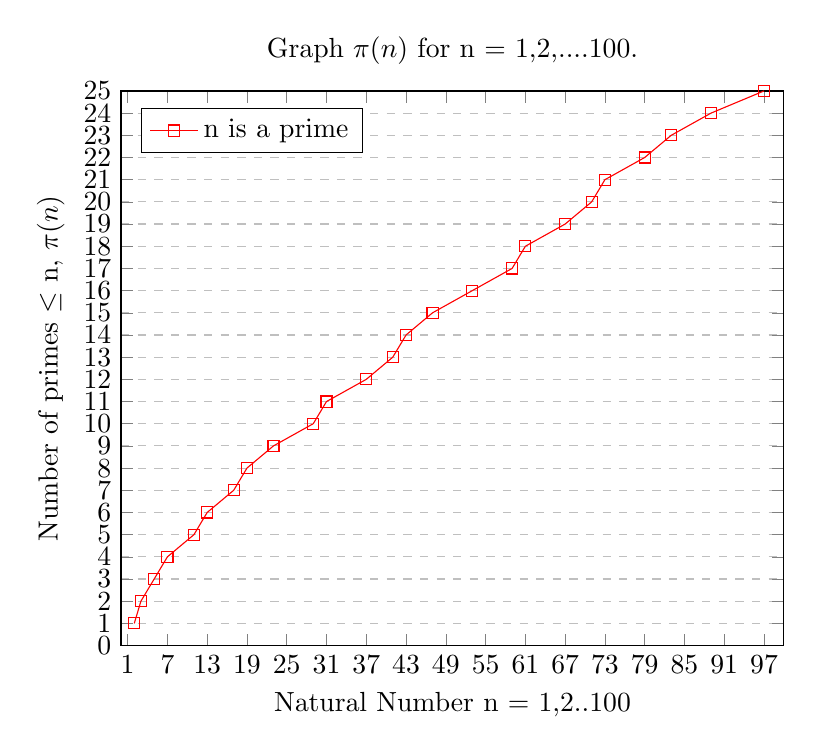
\begin{tikzpicture}
    \begin{axis}[
        title={Graph $\pi(n)$ for n = 1,2,....100.},
        xlabel={Natural Number n = 1,2..100},
        ylabel={Number of primes $\leq$ n, $\pi(n)$},
        xmin=0, xmax=100,
        ymin=0, ymax=25,
        xtick={1,7,13,19,25,31,37,43,49,55,61,67,73,79,85,91,97},
        ytick={0,1,2,3,4,5,6,7,8,9,10,11,12,13,14,15,16,17,18,19,20,21,22,23,24,25},
        legend pos=north west,
        ymajorgrids=true,
        grid style=dashed]
    \addplot[
        color=red,
        mark=square,
        ]
        coordinates {
        (2,1)(3,2)(5,3)(7,4)(11,5)(13,6)(17,7)(19,8)(23,9)(29,10)(31,11)(37,12)(41,13)(43,14)(47,15)(53,16)(59,17)(61,18)(67,19)(71,20)(73,21)(79,22)(83,23)(89,24)(97,25)
        };
        \legend{n is a prime}
    \end{axis}
\end{tikzpicture}

The relation between $\pi(n)$ and n is linear and $\pi(n)$ is approximately 25\% relative top n. The function $\frac{\pi(n)}{n}$ is generally a decreasing function. It approaches 0.\\
\textbf{Conjecture.} \textit{For each natural number n, define $\pi(n)$ to be the number of primes less than or equal to n. Then $\frac{\pi(n)}{n}$ is a decreasing function and it approaches 0 when n goes to infinity.}\\
To prove this conjecture we must prove that $\pi(n) \leq n, \forall n \in [1,2...100]$. This is true since the number of primes is always less than 100 in n. As the graph shows, when n is 97, the total number of prime is 25. For each prime n, we can see that each $\pi(n)$ is less than or equal to that prime n.  

\subsection*{2.7 Theorem (Fundamental Theorem of Arithmetic - Existence Part)} 
\quad \textit{Every natural number greater than 1 is either prime number or it can be expressed as finite product of prime numbers. That is, for every natural number n greater than 1, there exist distinct primes $p_1, p_2,....p_m$ and natural numbers $r_1,r_2,....r_m$ such that}

\begin{center}
    $n=p_{1}^{r_1}p_{2}^{r_2}...p_{m}^{r_m}$
\end{center}

\begin{proof}
\textbf{Base case (n = 1):  }
    \begin{flalign*}
        && n &= p_{1}^{r_1}p_{2}^{r_2}...p_{m}^{r_m} &&\\
        && 2 &= 2^1
    \end{flalign*}
    Thus making the theorem true for n = 2, the smallest possible prime.\\
\textbf{Inductive Hypothesis: } Assume n = n + 1, then Theorem still holds.\\ 
\textbf{Inductive Step: }
    \begin{itemize}
        \item If n + 1 is prime $\Longrightarrow n+1 = (n+1)^1$. Thus making the Theorem hold.
        \item If n + 1 is composite $\longrightarrow n+1 = xy, \exists x,y \in \mathbf{Z}, 1< x \leq y < n + 1$\\
        Let $x = p_{1}^{r_1}p_{2}^{r_2}...p_{m}^{r_m}$ and $y = q_{1}^{t_1}q_{2}^{t_2}...q_{m}^{t_m}$. Thus making,
        \begin{center}
            $n+1 = xy = p_{1}^{r_1}p_{2}^{r_2}...p_{m}^{r_m} \cdot q_{1}^{t_1}q_{2}^{t_2}...q_{m}^{t_m}$
        \end{center}
    \end{itemize}
    Therefore, the Theorem holds for all natural numbers greater than 1 and prime or composite.
\end{proof}

\subsection*{2.8 Lemma} 
\quad \textit{Let $p$ and $q_1,q_2,...,q_n$ all be primes and let k be a natural number such that $pk = q_1q_2...q_n$. Then $p=q_i$ for some i.}

\begin{proof}
By contradiction, suppose $p \neq q_i, \exists i \in [1,2...n]$. Since $p$ and $q_1,q_2,...,q_n$ are all be primes then $\gcd(p,q_i) = 1$. This implies that k is a rationale number since $k = \frac{q_1q_2...q_n}{p}$. Therefore, $p=q_i$ for some i to make k a natural number.
\end{proof}

\subsection*{2.9 Theorem (Fundamental Theorem of Arithmetic - Uniqueness part)}
\quad \textit{Let n be a natural number. Let \{$p_1,p_2,....,p_m$\} and \{$q_1,q_2,....,1_s$\} be sets of primes with $p_i \neq p_j$ if $i \neq j$ and $q_i \neq q_j$ if $i \neq j$. Let \{$r_1,r_2,....,r_m$\} and \{$t_1,t_2,....,t_m$\} be sets of natural numbers such that}

\begin{center}
    $n = p_{1}^{r_1}p_{2}^{r_2}...p_{m}^{r_m} = q_{1}^{t_1}q_{2}^{t_2}...q_{m}^{t_m}$
\end{center}

\textit{Then m = s and $\{p_{1},p_{2},...p_{m}\} = \{q_{1},q_{2},...q_{m}\}$. That is, the sets of primes are equal but their elements are not necessarily listed in the same order; that is, $p_i$ may or may not equal $q_i$. Moreover, if $p_i = q_j$ then $r_i=t_j$. In other words, if we express the same natural number as a product of powers of distinct primes, then the expressions are identical except for the ordering of the factors.}

\begin{proof}
If $n = p_{1}^{r_1}p_{2}^{r_2}...p_{m}^{r_m} = q_{1}^{t_1}q_{2}^{t_2}...q_{m}^{t_m}$, then assume that $k_i = p_{1}^{r_1}p_{2}^{r_2}...p_{m}^{r_m} \Longrightarrow n = p_ik_i = q_{1}^{t_1}q_{2}^{t_2}...q_{m}^{t_m}$.\\
By 2.8 Lemma, we can say that $p_i = p_j$. Since, $p_i \neq p_j, q_i \neq q_j, i \neq j$, we can state that $p_i = q_j$ then $r_i=t_j$ for any $p_i$ there is some $q_j$. As well as that m = s and $\{p_{1},p_{2},...p_{m}\} = \{q_{1},q_{2},...q_{m}\}$ where there exist a different $p_j$ for any $q_i$.
\end{proof}

\subsection*{2.10 Exercise} 
\quad \textit{Express $n=12!$ as a product of primes.}
\begin{flalign*}
    && n = 12! &= 1 \cdot 2 \cdot 3 \cdot 4 \cdot 5 \cdot 6 \cdot 7 \cdot 8 \cdot 9 \cdot 10 \cdot 11 \cdot 12&&\\
    && n = 12! &= 1 \cdot 2 \cdot 3 \cdot 2(2) \cdot 5 \cdot 2(3) \cdot 7 \cdot 2(2)(2) \cdot 3(3) \cdot 2(5) \cdot 11 \cdot 3(3)(3)(3)&&\\
    && n = 12! &= 1 \cdot 2^8 \cdot 3^8 \cdot 5^2 \cdot 7 \cdot 11&&
\end{flalign*}

\subsection*{2.11 Exercise} 
\quad \textit{Determine the number of zeros at the end of $25!$.}\\
Find the nearest factor of 5 that is less or equal to 25. In this case, it is 25. We divide perform $25 \div 5 = 5$, then we divide the quotient with 5 again until we can't anymore. $5 \div 5 = 1$. We then sum all the quotients, $5+1 =6$. Thus there will be 6 trialling zeros at the end of 25!.

\subsection*{2.12 Theorem} 
\quad \textit{Let a and b be natural numbers greater than 1 and let $p_{1}^{r_1}p_{2}^{r_2}...p_{m}^{r_m}$ be the unique factorization of a and let $q_{1}^{t_1}q_{2}^{t_2}...q_{m}^{t_m}$ be the unique prime factorization of b. Then $a \mid b$ if and only if for all $i \leq m$ there exits a $j \leq s$ such that $p_i = q_j$ and $r_i \leq t_j$.}

\begin{proof}
Assume $a \mid b$, then $a \mid b \Longrightarrow b = ka, \exists k \in \mathbf{Z}$. By Lemma 2.8, if $b = q_{1}^{t_1}q_{2}^{t_2}...q_{m}^{t_m}$ and $a = p_{1}^{r_1}p_{2}^{r_2}...p_{m}^{r_m}$, then $b = ka$ where k is some natural number and $p = q_i$ for some i. Since natural numbers are also a part of integers, $a \mid b$ still holds.
\end{proof}

\subsection*{2.13 Theorem} 
\quad \textit{If a and b are natural numbers and $a^2 \mid b^2$, then $a \mid b$.}

\begin{proof}
Since $a^2 \mid b^2$, we can express it as $b^2 = a^2k$ where since $b^2$ is a perfect square, thus making $a^2k$ also a perfect square. Assume, $k = p^2$.
\begin{flalign*}
    && b^2 &= a^2k &&\\ 
    && b^2 &= a^2p^2 &&\\ 
    && b^2 &= (ap)^2 &&\\ 
    && b &= (ap) &&\\
    && &\Longrightarrow a \mid b 
\end{flalign*}
\end{proof}

\subsection*{2.14 Exercise} 
\quad \textit{Find $(3^{14} \cdot 7^{22} \cdot 11^5 \cdot 17^3, 5^2 \cdot 11^4 \cdot 13^8 \cdot 17)$.}

\begin{center}
    $\gcd(3^{14} \cdot 7^{22} \cdot 11^5 \cdot 17^3, 5^2 \cdot 11^4 \cdot 13^8 \cdot 17) = 11^4 \cdot 17$
\end{center}

\subsection*{2.15 Exercise} 
\quad \textit{Find $lcm(3^{14} \cdot 7^{22} \cdot 11^5 \cdot 17^3, 5^2 \cdot 11^4 \cdot 13^8 \cdot 17)$.}

\begin{center}
    $lcm(3^{14} \cdot 7^{22} \cdot 11^5 \cdot 17^3, 5^2 \cdot 11^4 \cdot 13^8 \cdot 17) = \frac{(3^{14} \cdot 7^{22} \cdot 11^5 \cdot 17^3)(5^2 \cdot 11^4 \cdot 13^8 \cdot 17)}{\gcd(3^{14} \cdot 7^{22} \cdot 11^5 \cdot 17^3, 5^2 \cdot 11^4 \cdot 13^8 \cdot 17) = 11^4 \cdot 17} = 3^{14} \cdot 5^2 \cdot 7^{22} \cdot 11^5 \cdot 13^8 \cdot 17^3$
\end{center}

\subsection*{2.16 Exercise} 
\quad \textit{Make a conjecture that generalizes the ideas from the 2 previous exercises.}

\textbf{Conjecture.} Finding the greatest common denominator of $(a,b) = \gcd(p_{1}^{r_1}p_{2}^{r_2}...p_{m}^{r_m}, q_{1}^{t_1}q_{2}^{t_2}...q_{m}^{t_m})$ is done by doing an intersection between the primes of each value.

\begin{center}
    $(a,b) = \gcd(p_{1}^{r_1}p_{2}^{r_2}...p_{m}^{r_m}, q_{1}^{t_1}q_{2}^{t_2}...q_{m}^{t_m}) = \{p_{1}^{r_1},p_{2}^{r_2}...,p_{m}^{r_m}\} \cap \{q_{1}^{t_1},q_{2}^{t_2}...,q_{m}^{t_m}\}$
\end{center}

\textbf{Conjecture.} Finding the least common factor of $lcm(a,b) = lcm(p_{1}^{r_1}p_{2}^{r_2}...p_{m}^{r_m}, q_{1}^{t_1}q_{2}^{t_2}...q_{m}^{t_m})$ is done by factoring the $\gcd(a,b)$ from the product of a and b.

\begin{center}
    $lcm(a,b) = lcm(p_{1}^{r_1}p_{2}^{r_2}...p_{m}^{r_m}, q_{1}^{t_1}q_{2}^{t_2}...q_{m}^{t_m}) = \frac{a \cdot b}{(a,b)}= \frac{p_{1}^{r_1}p_{2}^{r_2}...p_{m}^{r_m} \cdot q_{1}^{t_1}q_{2}^{t_2}...q_{m}^{t_m}}{\gcd(p_{1}^{r_1}p_{2}^{r_2}...p_{m}^{r_m}, q_{1}^{t_1}q_{2}^{t_2}...q_{m}^{t_m})}$
\end{center}

\subsection*{2.17 Question} 
\quad \textit{Do you think this method is always better, always worse, or sometimes better and sometimes worse than using the Euclidean Algorithm to find (a,b)? Why?}\\
I find that this method is sometimes worse than using the Euclidean Algorithm since we need to find all primes for each a and b which can take longer than using the Euclidean Algorithm.

\subsection*{2.18 Theorem} 
\quad \textit{Given n+1 natural numbers, say $a_1,a_2,...,a_n+1$, all less than or equal to 2n, then there exists a pair, say $a_i$ and $a_j$ with $i \neq j$, such that $a_i \mid a_j$.}

\begin{proof}
\textbf{Base case (n = 1):  }
    Then for natural number 1+1=2, there exist $a_1$ and $a_2$ all less than or equal to 2(1). $a_1 = 1 \leq 2(1)$ and $a_2 = 2 \leq 2(1)$. Also $a_i \mid a_j \Longrightarrow 1 \mid 2$, thus making the theorem hold for n = 1.\\
\textbf{Inductive Hypothesis: } Assume $n + 1 = k$, then Theorem still holds for $k + 1$.\\ 
\textbf{Inductive Step: }
    For the natural number, $(k+1)+1 = k + 2$, there exist $a_1,a_2,...,a_k+1$, all less than or equal to $2(k+1) = 2k + 2$, then there exists a pair, say $a_i$ and $a_j$ with $i \neq j$, such that $a_i \mid a_j$.
    \begin{itemize}
        \item If $a_1,a_2,...,a_k+1$ numbers for $k+2$ are less than or equal to $2(k+1)$. Then the hypothesis still holds.
        \item If $a_1,a_2,...,a_k+1$ numbers for $k+2$ are \textbf{not} less than or equal to $2(k+1)$. Then $a_1,a_2,...,a_k+1$ numbers must be $2(k+1)+1, 2(k+1)+2,...2(k+1)+k+1$. Then, $2(k+1)+1 \nmid 2(k+1)+2$ and $2(k+1)+2 \nmid 2(k+1)+k+1$. Thus, by contradiction, all $a_1,a_2,...,a_k+1$ numbers for $k+2$ must be less than or equal to $2(k+1)$.
    \end{itemize}
    Therefore, the Theorem holds for n + 1 natural numbers where $a_1,a_2,...,a_n+1$ are all less than or equal to 2n.
\end{proof}

\subsection*{2.19 Theorem} 
\quad \textit{There do not exist natural numbers m and n such that $7m^2 = n^2$.}

\begin{proof}
By Fundamental Theorem of Arithmetic, let $m = p_{1}^{r_1}p_{2}^{r_2}...p_{m}^{r_m}$ and $n = q_{1}^{t_1}q_{2}^{t_2}...q_{m}^{t_m}$. Thus $7m^2 = n^2 \Longrightarrow 7 \cdot p_{1}^{2r_1}p_{2}^{2r_2}...p_{m}^{2r_m} = q_{1}^{2t_1}q_{2}^{2t_2}...q_{m}^{2t_m}$. Since, all p and q are prime numbers, the left hand side will always have an extra prime number of 7, thus making the min total number of the prime 7 to the power of 3 (an odd number), $7^3$. The right hand side will always have the prime 7 to the power of a even number (min of 2). Thus, $7m^2 \neq n^2 \Longrightarrow 7 \cdot p_{1}^{2r_1}p_{2}^{2r_2}...p_{m}^{2r_m} \neq q_{1}^{2t_1}q_{2}^{2t_2}...q_{m}^{2t_m}$.
\end{proof}

\subsection*{2.20 Theorem} 
\quad \textit{There do not exist natural numbers m and n such that $24m^3 = n^3$.}

\begin{proof}
By Fundamental Theorem of Arithmetic, let $24m^3 = n^3 \Longrightarrow (3 \cdot 2^3) \cdot p_{1}^{3r_1}p_{2}^{3r_2}...p_{m}^{3r_m} = q_{1}^{3t_1}q_{2}^{3t_2}...q_{m}^{3t_m}$. Then,
    \begin{flalign*}
        && (3 \cdot 2^3) \cdot p_{1}^{3r_1}p_{2}^{3r_2}...p_{m}^{3r_m} &= q_{1}^{3t_1}q_{2}^{3t_2}...q_{m}^{3t_m} &&\\
        && (3 \cdot 2^3)  &= \frac{p_{1}^{3r_1}p_{2}^{3r_2}...p_{m}^{3r_m}}{q_{1}^{3t_1}q_{2}^{3t_2}...q_{m}^{3t_m}} &&\\
        && (3 \cdot 2^3)  &= \frac{p_{1}^{r_1}p_{2}^{r_2}...p_{m}^{r_m}}{q_{1}^{t_1}q_{2}^{t_2}...q_{m}^{t_m}}^3 &&\\
        && (3 \cdot 2^3)  &= k^3 && k = \frac{p_{1}^{r_1}p_{2}^{r_2}...p_{m}^{r_m}}{q_{1}^{t_1}q_{2}^{t_2}...q_{m}^{t_m}}, k is prime \\
        && (3^{\frac{1}{3}} \cdot 2) &= k &&\\
        && 3^{\frac{1}{3}} &= \frac{k}{2} &&
    \end{flalign*}
    There are no possible prime values of k where $\frac{k}{2} = 3^{\frac{1}{3}}$. Thus by contradiction, $24m^3 \neq n^3$. As well as, given $24m^3 = n^3 \Longrightarrow 24 = \frac{n^3}{m^3} = k^3 \Longrightarrow 24^{\frac{1}{3}} = k$, $24^{\frac{1}{3}}$ does not result into a prime number.  
\end{proof}

\subsection*{2.21 Exercise} 
\quad \textit{Show that $\sqrt{7}$ is irrational. That is, there do not exist natural numbers n and m such that $\sqrt{7} = \frac{m}{n}$.}

\begin{proof}
    \begin{flalign*}
        &&\sqrt{7} &= \frac{m}{n} &&\\
        &&7^{\frac{1}{2}} &= \frac{m}{n} &&\\
        &&7 &= \frac{m}{n}^2 &&\\
        &&7 &= \frac{m^2}{n^2} &&\\
        &&7 \cdot n^2 &= m^2
    \end{flalign*}
    By Theorem 2.9, $7 \cdot n^2 \neq m^2$. Therefore, there do not exist natural numbers n and m.
\end{proof}

\subsection*{2.22 Exercise} 
\quad \textit{Show that $\sqrt{12}$ is irrational.}

\begin{proof}
    \begin{flalign*}
        && &\Longrightarrow \sqrt{12} &&\\
        && &\Longrightarrow \sqrt{2^2 \cdot 3} &&\\
        && &\Longrightarrow 2 \cdot \sqrt{3}
    \end{flalign*}
    The square root of prime is an irrational number thus $\sqrt{3}$ is irrational which also makes $2 \cdot \sqrt{3}$ irrational.
\end{proof}

\subsection*{2.23 Exercise} 
\quad \textit{Show that $7^{\frac{1}{3}}$ is irrational.}

\begin{proof}
Since 7 is prime, then $7^{\frac{1}{3}}$ is irrational since cubic root of a prime results in a non real natural number thus making them irrational.
\end{proof}

\subsection*{2.24 Question} 
\quad \textit{What other numbers can you show to be irrational? Make and prove the most general conjecture you can.}

Any prime number to a root results into an irrational number.\\
\textbf{Conjecture.} For any prime p, $p^{\frac{1}{k}}, \forall k \in \mathbf{Z}$ will result to a irrational number.

\subsection*{2.25 Theorem} 
\quad \textit{Let a, b, and n be integers. If $a \mid n$, $b \mid n$, and $(a,b) = 1$, then $ab \mid n$.}

\begin{proof}
Since $a \mid n$ and $b \mid n$, we can state that $ n = sa = kb, \exists s,k \in \mathbf{Z}$. Since the $\gcd(a,b) = 1$, then a and b can not divide each other and that $ax + by = 1$ for some integer x and y. By Fundamental Theorem of Arithmetic, n can be expressed in the product of prime numbers and so does s and k. Thus suppose $n = p_{1}^{r_1}p_{2}^{r_2}...p_{m}^{r_m} \cdot a = q_{1}^{t_1}q_{2}^{t_2}...q_{m}^{t_m} \cdot b$.

\begin{flalign*}
    && ax + by &= 1 &&\\
    && axn + byn &= n &&\text{Multiplying n in both sides}\\
    && ax(q_{1}^{t_1}q_{2}^{t_2}...q_{m}^{t_m} \cdot b) + by(p_{1}^{r_1}p_{2}^{r_2}...p_{m}^{r_m} \cdot a) &= n &&\text{Defining n}\\
    && ab (xq_{1}^{t_1}q_{2}^{t_2}...q_{m}^{t_m} + yp_{1}^{r_1}p_{2}^{r_2}...p_{m}^{r_m}) &= n &&
\end{flalign*}
Thus making $ab \mid n$.
\end{proof}

\subsection*{2.26 Theorem} 
\quad \textit{Let p be a prime and let a be an integer. Then p does not divide a if and only if $(a,p) = 1$.}

\begin{proof}
Lets say that $(a,p) = b \neq 1$. Then, $b \mid a$ and $b \mid p$. Since p is prime b can either be 1 or p. But, by contradiction, $b \neq 1$, thus $b = p$. Also, since  $b \mid a \Longrightarrow p \mid a$, but p does not divide a. Meaning that, b must be 1.
\end{proof}

\subsection*{2.27 Theorem} 
\quad \textit{Let p be a prime and let a and b be integers. If $p \mid ab$, then $p \mid a$ or $p \mid b$.}

\begin{proof}
If $p \mid ab$, then $ab = kp, \exists k \in \mathbf{Z}$. Therefore, $k = \frac{ab}{p}$. Since k is an integer, p must divide either a or b.
\end{proof}

\subsection*{2.28 Theorem} 
\quad \textit{Let a, b, and c be integers. If $(b,c) = 1$, then $(a,bc) = (a,b) \cdot (a,c)$.}

\begin{proof}
    \begin{flalign*}
        && (a, bc) &= (a,b) \cdot (a,c) &&\\
        && (a, bc) &= (ax + by) \cdot (am + cn) && \text{For some integer x,y,m and n}\\
        && (a, bc) &= (ax + by) \cdot (am + cn) &&\\
        && (a, bc) &= axam + axcn + byam + bycn &&\\
        && (a, bc) &= a(xm + xcn + bym) + bc(yn) &&\\
        && (ap + bq) &= a(xm + xcn + bym) + bc(yn) &&\\
        && (a, bc) &= (a, bc) &&\text{Where p = xm + xcn + bym and q = yn}\\ 
    \end{flalign*}
    Thus $(a,bc) = (a,b) \cdot (a,c)$ if b and c do not divide each other.
\end{proof}

\begin{proof}
Given $(b,c) = 1$, then b and c have no common primes that make them up. (a,bc) suggests that there are common primes that make up a and bc (by fundamental theorem of arithmetic). (a,b) gives common primes that make up a and b but not c. Hence, (a,c) gives common primes that make up a and c but not b. Therefore, if we do $(a,b) \cdot (a,c)$, we would get common prime that make up a and primes that would make up b*c.
\end{proof}

\subsection*{2.29 Theorem} 
\quad \textit{Let a, b, and c be integers. If $(a,b) = 1$ and $(a,c) = 1$, then $(a,bc) = 1$.}

\begin{proof}Given the following,
    \begin{itemize}
        \item $(a,b) = 1 \Longrightarrow ax + by = 1, \exists x,y \in \mathbf{Z}$
        \item $(a,c) = 1 \Longrightarrow am + cn = 1, \exists m,n \in \mathbf{Z}$
        \item $(a,bc) = 1 \Longrightarrow as + bct = 1, \exists s,t \in \mathbf{Z}$
    \end{itemize}
    Then,
    \begin{flalign*}
        && as + bct &= 1 &&\\
        && as + bt(\frac{1-am}{n}) &= 1 &&\\
        && as + b(\frac{t-amt}{n}) &= 1 &&
    \end{flalign*}
    Similarly,
    \begin{flalign*}
        && as + bct &= 1 &&\\
        && as + ct(\frac{1-ax}{y}) &= 1 &&\\
        && as + c(\frac{t-axt}{y}) &= 1 &&
    \end{flalign*}
    Thus, If $(a,b) = 1$ and $(a,c) = 1$, then $(a,bc) = 1$.
\end{proof}
    
\begin{proof}
    By fundamental theorem of arithmetic, a, b and c are made up of primes. If that $(a,b) = 1$, then there are no common primes that make up a and b. Similarly, $(a,c) = 1$ suggests that there are no common primes that make up either a and c. Hence, there can not be any common primes between a, b and c. Same for a and bc, thus (a,bc) = 1.
\end{proof}

\subsection*{2.30 Theorem} 
\quad \textit{Let a and b integers. If $(a,b) = d$, then $(\frac{a}{d},\frac{b}{d}) = 1$.}

\begin{proof}Given the following,
    \begin{itemize}
        \item $(a,b) = d \Longrightarrow ax + by = d, \exists x,y \in \mathbf{Z}$
        \item $(\frac{a}{d},\frac{b}{d}) = 1 \Longrightarrow \frac{am}{d} + \frac{bn}{d} = 1, \exists m,n \in \mathbf{Z}$
    \end{itemize}
    Thus, $\frac{am}{d} + \frac{bn}{d} = 1 \Longrightarrow a\frac{m}{d} + b\frac{n}{d} = 1$ then $x = \frac{m}{d}$ and $y = \frac{n}{d}$.
\end{proof}

\begin{proof}
By fundamental theorem of arithmetic, a, and d are all made up of primes. Given (a,b) = d, d is the common primes that make up a and b. Then $\frac{a}{d}$ results to the primes that are not common to a and b. Similarly, $\frac{b}{d}$ results to the primes that are not common to a and b. Therefore $\frac{a}{d}$ and $\frac{b}{d})$ have no common primes thus $(\frac{a}{d},\frac{b}{d}) = 1$.
\end{proof}

\subsection*{2.31 Theorem} 
\quad \textit{Let a, b, u, and v be integers. If $(a,b) = 1$ and $u \mid a$ and $v \mid b$, then $(uv) = 1$.}

\begin{proof}Given the following,
    \begin{itemize}
        \item $(a,b) = 1 \Longrightarrow ax + by = 1, \exists x,y \in \mathbf{Z}$
        \item $u \mid a \Longrightarrow a = ku, \exists u \in \mathbf{Z}$
        \item $v \mid b \Longrightarrow b = sv, \exists v \in \mathbf{Z}$
    \end{itemize}
    \begin{flalign*}
        && ax + by &= 1 &&\\
        && (ku)x + (sv)y &= 1 &&\\
        && u(kx) + v(sy) &= 1 &&\\
    \end{flalign*}
    Thus, $(uv) = 1$.
\end{proof}

\begin{proof}
By fundamental theorem of arithmetic, a, b, u, and v are made up of primes. If $(a,b) = 1$ implies that a and b have no common primes. $u \mid a$ and $v \mid b$ imply that a is formed by u's primes and b is formed by v's primes. Therefore, u and v do not have any similar prime i.e. $(uv) = 1$.
\end{proof}

\subsection*{2.32 Theorem} 
\quad \textit{For all natural numbers n, $(n, n+1) = 1$.}

\begin{proof}
    \textbf{Base case (n = 1):  }
    \begin{flalign*}
        && (n,n+1) &= 1 &&\\
        && (1,2) &= 1 &&\\
    \end{flalign*}
    Theorem holds for n = 1.\\
\textbf{Inductive Hypothesis: } Assume n = n + 1, then Theorem still holds.\\ 
\textbf{Inductive Step: }
     \begin{flalign*}
        && (n,n+1) &= 1 &&\\
        && (n+1,n+2) &= 1 &&\\
        && (n+1)x + (n+2)y &= 1 && \text{For some integer x and y.}\\
        && nx + x + ny + 2y &= 1 &&\\
        && n(x + y) + 1(x + 2y) &= 1 &&\\
        && (n,1) &= 1 &&\\
    \end{flalign*}
    Therefore, the theorem still holds.
\end{proof}

\subsection*{2.33 Theorem} 
\quad \textit{Let k be a natural number. Then, there exists a natural number n (which will be much larger than k) such that no natural number less than k and greater than 1 divides n.}

\begin{proof}
Let there exists a natural number k, n and s such $k < n$ and $1 < s < k$ and s is a prime. By contradiction, if $k \mid n$ and $s \nmid k$. Then $s \nmid n$.
\end{proof}

\subsection*{2.34 Theorem} 
\quad \textit{Let k be a natural number. Then there exists a prime larger than k.}

\begin{proof}
By Theorem 2.32, for all natural numbers n, (n,n+ 1) = 1, let p be a prime and a natural number, then there will be $(p_n, p_s) = 1, p_n = p_1$. There will be a $p_n+1$ that will be prime.

\begin{proof}
    \textbf{Base case (n = 2) (Lowest possible prime):  }
    \begin{flalign*}
        && (2,3) &= 1 &&\\
        && (2,3) &= 1 &&\\
    \end{flalign*}
    n + 1 is a prime.\\
\textbf{Inductive Hypothesis: } Assume n = n + 1, then Theorem still holds with any any prime.\\ 
\textbf{Inductive Step: }
     \begin{flalign*}
        && (n,n+1) &= 1 &&\\
        && (n+1,n+2) &= 1 &&\\
        && (n+1)x + (n+2)y &= 1 && \text{For some integer x and y.}\\
        && nx + x + ny + 2y &= 1 &&\\
        && n(x + y) + 1(x + 2y) &= 1 &&\\
        && (n,1) &= 1 &&\\
    \end{flalign*}
    The gcd of a prime with 1 will always be 1, therefore the theorem holds.
\end{proof}

\end{proof}

\subsection*{2.35 Theorem (Infinitude of Primes Theorem)} 
\quad \textit{There are infinitely many prime numbers.}

\begin{proof}
Let P be a finite set of primes, $ P = \{ p_{1},p_{2}...p_{m}\}$. We need to show that there will be prime numbers not in P. Now let q be the product of all elements in the set P such that $q = p_{1}p_{2}...p_{m}$. By Theorem 2.32, we know that for all natural numbers n, (n, n+1) = 1 such that n and n+1 are co primes. Therefore, (q, q+1) = 1, meaning that there is a number $x$ that divides $q+1$ that is not in the finite prime set P.
\end{proof}

\subsection*{2.36 Question} 
\quad \textit{What were the most clever or most difficult parts in your proof of the infinitude of Primes Theorem?}

The most clever way was by using Theorem 3.32. This shows that there is a continuity of co-primes and thus helping show the Infinitude of Primes.

\subsection*{2.37 Theorem} 
\quad \textit{If $r_1,r_2,...,r_m$ are natural numbers and each one is congruent to 1 modulo 4, then the product $r_1r_2...r_4$ is also congruent to 1 modulo 4.}

\begin{proof}
By Euclidean Algorithm we can say that for each r,
    \begin{flalign*}
        && r_1 &= 1 + 4n_1 && \text{For some integer $n_1$}\\
        && r_2 &= 1 + 4n_2 && \text{For some integer $n_2$}\\
        && ... &= ... &&\\
        && r_m &= 1 + 4n_m && \text{For some integer $n_m$}\\
    \end{flalign*}
    The product of $r_1r_2...r_4$ will then result to
    \begin{flalign*}
        & \Longrightarrow (1 + 4n_1)(1 + 4n_2)...(1 + 4n_m) &&\\
        & \Longrightarrow 1 + 4(n_1+n_2+...n_m) + 4^2(n_1+n_2+...n_m) + ... + 4^m(n_1+n_2+...n_m)&&\\
        & \Longrightarrow 1 + 4 ((n_1+n_2+...n_m) + 4(n_1+n_2+...n_m) + ... + 4^{m-1}(n_1+n_2+...n_m))&&\\
        & \Longrightarrow 1 + 4x&&
    \end{flalign*}
    (For some integer x, where $x = (n_1+n_2+...n_m) + 4(n_1+n_2+...n_m) + ... + 4^{m-1}(n_1+n_2+...n_m)$)\\
    Thus the product $r_1r_2...r_4$ is also congruent to 1 modulo 4.
\end{proof}

\subsection*{2.38 Theorem (Infinitude of 4k + 3 Primes Theorem)}
\quad \textit{There are infinitely many prime numbers that are congruent to 3 modulo 4.}

Suppose, by contradiction, that there are a finite number of prime numbers that are congruent to 3 modulo 4. Let the set of $\{q_1, q_2,...,q_s\}, s < \infty$ and each $q_s \equiv 3 \bmod 4$. Now let the product of all $q_1 \cdot q_2 \cdot ... \cdot q_s = Q$.\\
Also, let $k \equiv 3 \bmod 4 \Longrightarrow k = 4 \cdot n -1$ and k is odd. By Fundamental Theorem of Arithmetic, n can be defined by the product of primes. Hence, let $n = Q = q_1 \cdot q_2 \cdot ... \cdot q_s$. Therefore,
\begin{center}
    $k = 4 \cdot q_1 \cdot q_2 \cdot ... \cdot q_s - 1$
\end{center}
Moreover, assuming k is not prime, then by fundamental theorem of arithmetic, k can be factored by primes such as $p_{1}^{2r_1}p_{2}^{2r_2}...p_{m}^{2r_m}$.\\

\subsection*{2.39 Question} 
\quad \textit{Are there other theorems like the previous one that you can prove?}

Well, it is not same but there is a finite number of primes that are congruent to 0 modulo 2, in fact only one. Also, there are infinitely many prime numbers that are congruent to 2 modulo 3.

\begin{proof}
Suppose, by contradiction, that there are a finite number primes that are congruent to 2 modulo 3, noted as $3, p_1, p_2,...,p_r, r < \infty$. Let P be the product of those primes with the addition of 2, $P = 3p_1p_2...p_r+2$. If P is prime, then P is congruent to 3 modulo 4 and it is not one of $3, p_1, p_2,...,p_r, r < \infty$.\\ However, if P is composite then, let $P = q_1q_2...q_s$. Note that not all $q$ are congruent to 2 modulo 3 since if so, then P should also be congruent. However, there must exist at least one $q$ that is congruent to 2 modulo 3. This $q$ can not be included in $3, p_1, p_2,...,p_r, r < \infty$ as if it was included, then $q$ would divide P and divide $4p_1p_2...p_r, r < \infty$. Thus making it divide the difference, which would be 3. If $q = 3$, then $q$ cannot divide $4p_1p_2...p_r, r < \infty$. By contradiction then, there must be an infinitely many prime numbers that are congruent to 2 modulo 3.\\
\end{proof}

\subsection*{2.40 Exercise} 
\quad \textit{Find the current record for the longest arithmetic progression of primes.}

The current record is $224584605939537911 + 81292139 \cdot 23 \cdot n, n = 0,..,26$ by Rob Gahan and PrimeGrid on 23 September 2019.

\subsection*{2.41 Exercise} 
\quad \textit{Use polynomial long division to compute $(x^m-1) \div (x-1)$.}

Unable to compute because of unknown value of m. If m is even, then it is doable by $(a+b)(a-b) = a^2-b^2$.

\subsection*{2.42 Theorem} 
\quad \textit{If n is a natural number and $2^n-1$ is prime, then n must be prime.}

\begin{proof}
Let $2^n-1$ be prime and n not prime and $n = ab, \exists a,b \in \mathbf{Z}$. 
    \begin{flalign*}
        &\Longrightarrow 2^n-1 &&\\
        &\Longrightarrow 2^{ab}-1 &&\\
        &\Longrightarrow (2^a-1^{b-1})^b &&\\
        &\Longrightarrow (2^a-1)(2^{a(b-1)}+...+2^a+1) &&\\
        &\Longrightarrow 2^a-1 \mid 2^n-1&&
    \end{flalign*}
    This is a contradiction, since $2^n-1$ is prime. Thus n must be prime.
\end{proof}

\subsection*{2.43 Theorem} 
\quad \textit{If n is a natural number and $2^n+1$ is prime, then n must be a power of 2.}

\begin{proof}
Let $2^n+1$ be prime and $n=2^k$. Suppose n has an odd factor $t > 1$. For all odd factors t, $x + 1 \mid x^t+1$ by the Root-Factor Theorem. Suppose $x = 2^{\frac{n}{t}} \Longrightarrow 2^{\frac{n}{t}}-1 \mid 2^n-1, 1 < 2^{\frac{n}{t}}-1 < 2^n-1$. Since, $2^n$ is prime, then n must have no odd factors and thus must be as power of 2.
\end{proof}

\subsection*{2.44 Exercise} 
\quad \textit{Find the first few Mersenne primes and Fermat primes.}\\

Mersenne Primes:
\begin{itemize}
    \item $2^{2} + 1 = 3$
    \item $2^{3} + 1 = 7$
    \item $2^{5} + 1 = 31$
    \item $2^{7} + 1 = 127$
    \item $2^{11} + 1 = 2049$
\end{itemize}
Fermat Primes:
\begin{itemize}
    \item $2^{2^0} + 1 = 3$
    \item $2^{2^1} + 1 = 5$
    \item $2^{2^2} + 1 = 17$
    \item $2^{2^3} + 1 = 257$
    \item $2^{2^4} + 1 = 65537$
\end{itemize}

\subsection*{2.45 Exercise} 
\quad \textit{For an A in the class and a Ph.D. in mathematics, prove that there are infinitely many Mersenne primes (or Fermat primes) or prove that there aren't.}

It is impossible to tell since there are an infinity number of primes.

\subsection*{2.46 Theorem} 
\quad \textit{There exist arbitrarily long strings of consecutive composite numbers. That is, for any natural number n there is a string of more than n consecutive composite numbers.}

\begin{proof}
By the Prime Number Theorem, as n approaches infinity, the number of primes less than n, $\pi(n)$, approaches $\frac{n}{\ln{n}}$, that is 
    \begin{center}
        $\lim\limits_{n\to \infty} {\frac{\pi(n)}{\frac{n}{\ln{n}}} = 1}$ 
    \end{center}
Therefore, as the number of primes decrease, there will be an arbitrary number of consecutive composite numbers.
\end{proof}

\subsection*{2.47 Question (The Twin Primes Question)}
\quad \textit{Are there infinitely many pairs of prime numbers that differ from one another by two? (The pairs 11 and 13, 29 and 31, 41 and 43 are examples of such twin primes.)}

Yes, since there is an infinite number of primes, there has to be a infinite number of primes as well.

\subsection*{2.48 Exercise} 
\quad \textit{Express each of the first 20 even numbers greater than 2 as a sum of two primes. (For example: $8 = 5+3$.)}

\begin{enumerate}
    \item $4 = 2 + 2$
    \item $6 = 2 + 3$
    \item $8 = 3 + 5$
    \item $10 = 5 + 5$
    \item $12 = 5 + 7$
    \item $14 = 7 + 7$
    \item $16 = 5 + 11$
    \item $18 = 7 + 11$
    \item $20 = 7 + 13$
    \item $22 = 5 + 17$
    \item $24 = 5 + 19$
    \item $26 = 7 + 19$
    \item $28 = 5 + 23$
    \item $30 = 11 + 19$
    \item $32 = 13 + 19$
    \item $34 = 3 + 31$
    \item $36 = 5 + 31$
    \item $38 = 7 + 31$
    \item $40 = 3 + 37$
    \item $42 = 5 + 37$
\end{enumerate}

\subsection*{2.49 Blank Paper Exercise} 
\begin{itemize}
    \item Fundamental Theorem of Primes
    \item Primes and GCD/LCM
    \item Irrational numbers
    \item Proofs using fundamental theorem of Primes
    \item infinite number of primes theorem
    \item infinity number of 4k+3 and ak+b primes
    \item Mersenne and Fermat Primes
    \item twin primes
    \item Goldbach Conjecture
\end{itemize}

\subsection*{2.50 Exercise} 
\quad \textit{Find the current record for the largest known Mersenne prime.}

The current record is held at 24,862,048 digits and the Mersenne prime is $2^{82,589,933}-1$.

\end{document}